\documentclass[slovak]{iamthesis}
% changle "slovak" to "english" for english version of the thesis


%----------------------------------------------------------------%
% THESIS DATA

% student name with title e.g. Ing. Martin Klaučo
\def\thesisauthor{Matej Kintler} 

% year of submmiting to AIS
\def\thesisyear{2020}

% registration number generated by AIS e.g. 19990-50920
\def\thesisnumber{FCHPT-5414-81521} 

% thesis type: BACHELOR|MASTER|DISSERTATION or in slovak 
% BAKALÁRSKA|DIPLOMOVÁ|DIZERTAČNÁ
\def\thesistype{DIPLOMOVÁ}

% thesis title
\def\thesistitle{Garantovaná identifikácia a jej využitie pre hybridné modelovanie}

% thesis supervisor including degrees e.g. Ing. Martin Klaučo, PhD.
\def\thesissupervisor{doc. Ing. Radoslav Paulen, PhD.}

% study field (translate to english if neccesarry) e.g. "Riadenie Procesov" or
% "Process Control"
\def\thesisprogram{Riadenie Procesov}

% Institute (translate to english if neccesary)
% e.g., "Institute of Information Engineering, Automation, and Mathematics"
\def\thesisinst{Oddelenie informatizácie a riadenia procesov}

% Title of the Acknowledgment
% For slovak write: "Poďakovanie" for English write: "Acknowledgment"
\def\thesisack{Poďakovanie}


% End THESIS DATA
%----------------------------------------------------------------%

%----------------------------------------------------------------%
%   Titles and other stuff                                       %
%----------------------------------------------------------------%
\author{\thesisauthor}
\title{\thesistitle}
\date{\today}
%\usepackage{layouts}
%\usepackage{layout}
%----------------------------------------------------------------%
%   Let the document begin                                       %
%----------------------------------------------------------------%
\begin{document}

% ---------------------------------------------------------------%
% The Frontmatter  !! Do NOT change the structure !!             % 
%----------------------------------------------------------------%

\coverpage

\frontmatter
\pagenumbering{roman}

% include assignment generated by AIS system
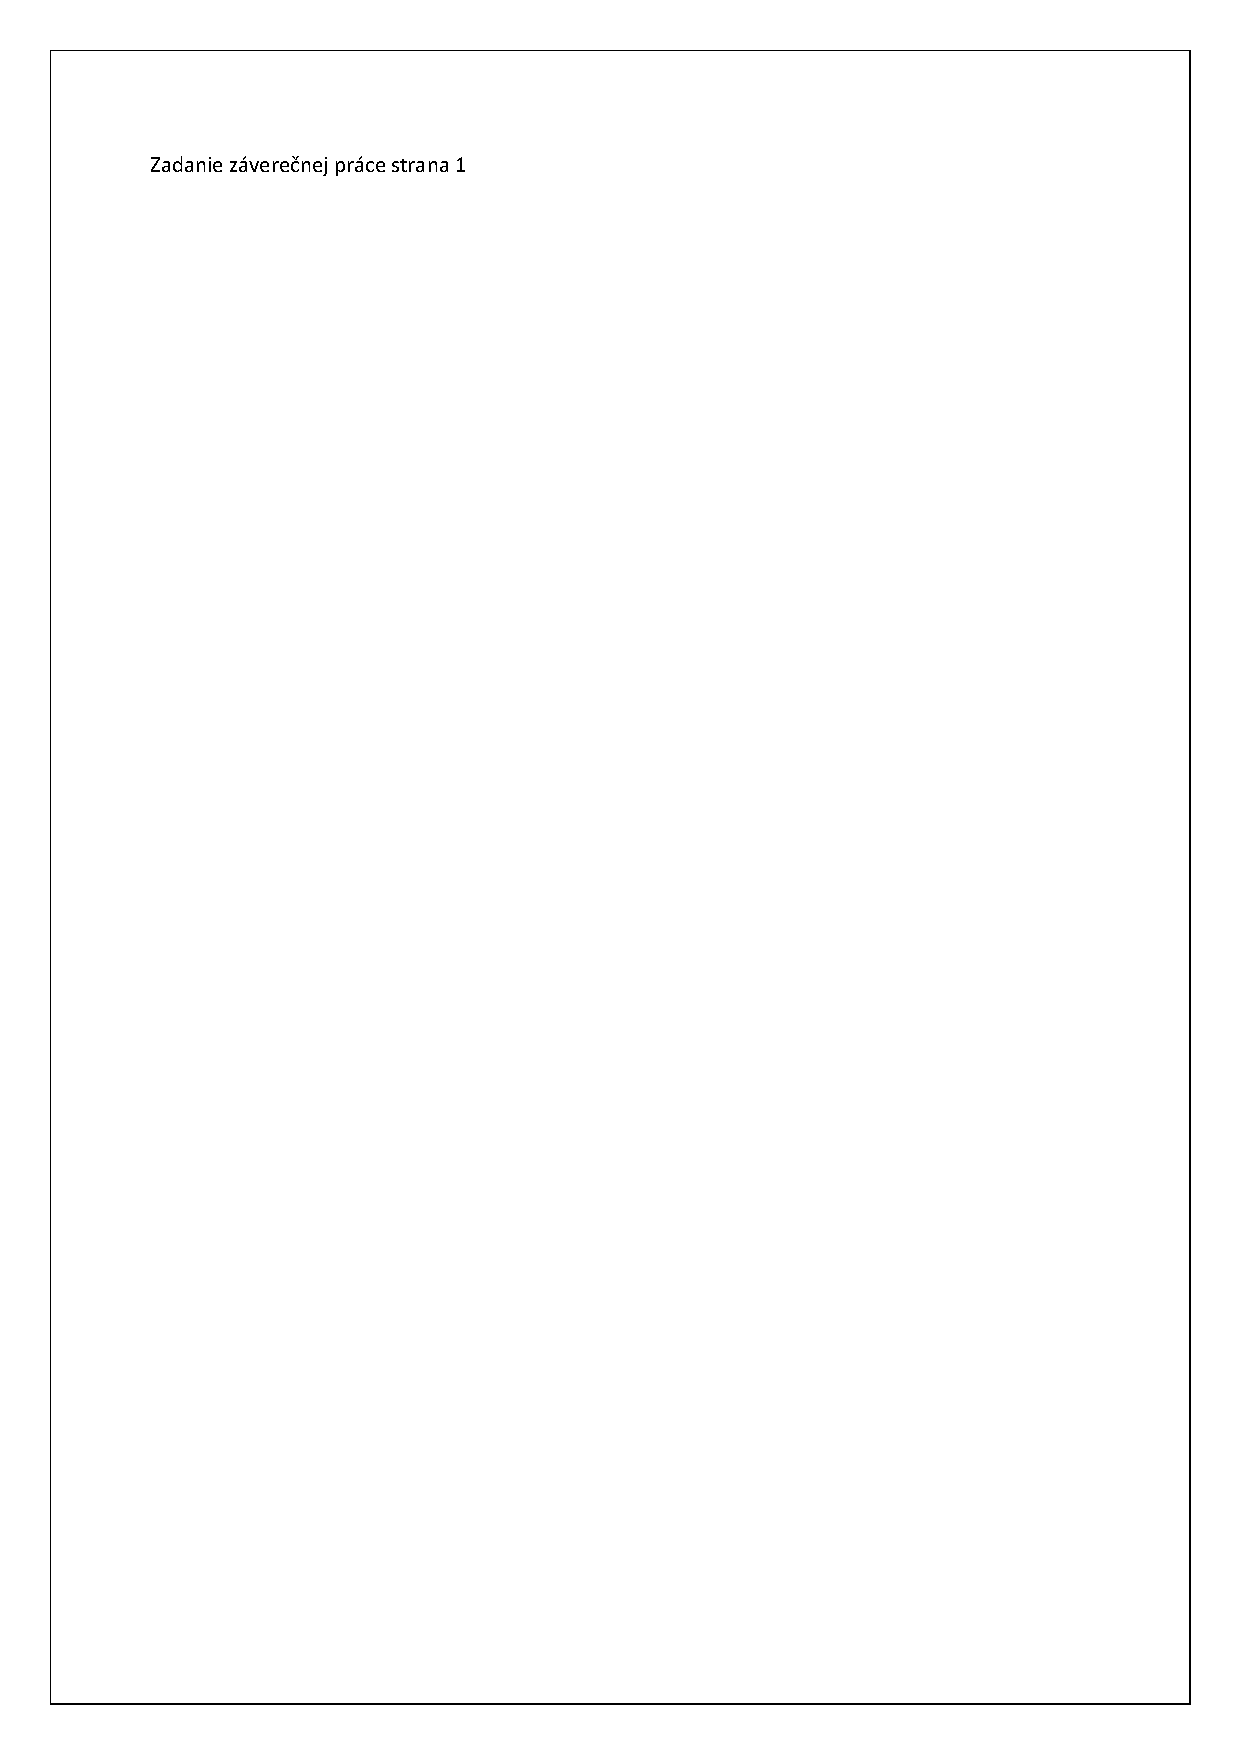
\includepdf[page=1]{content/assignment.pdf}
% use this command only if your assignment has more than 2 pages
% 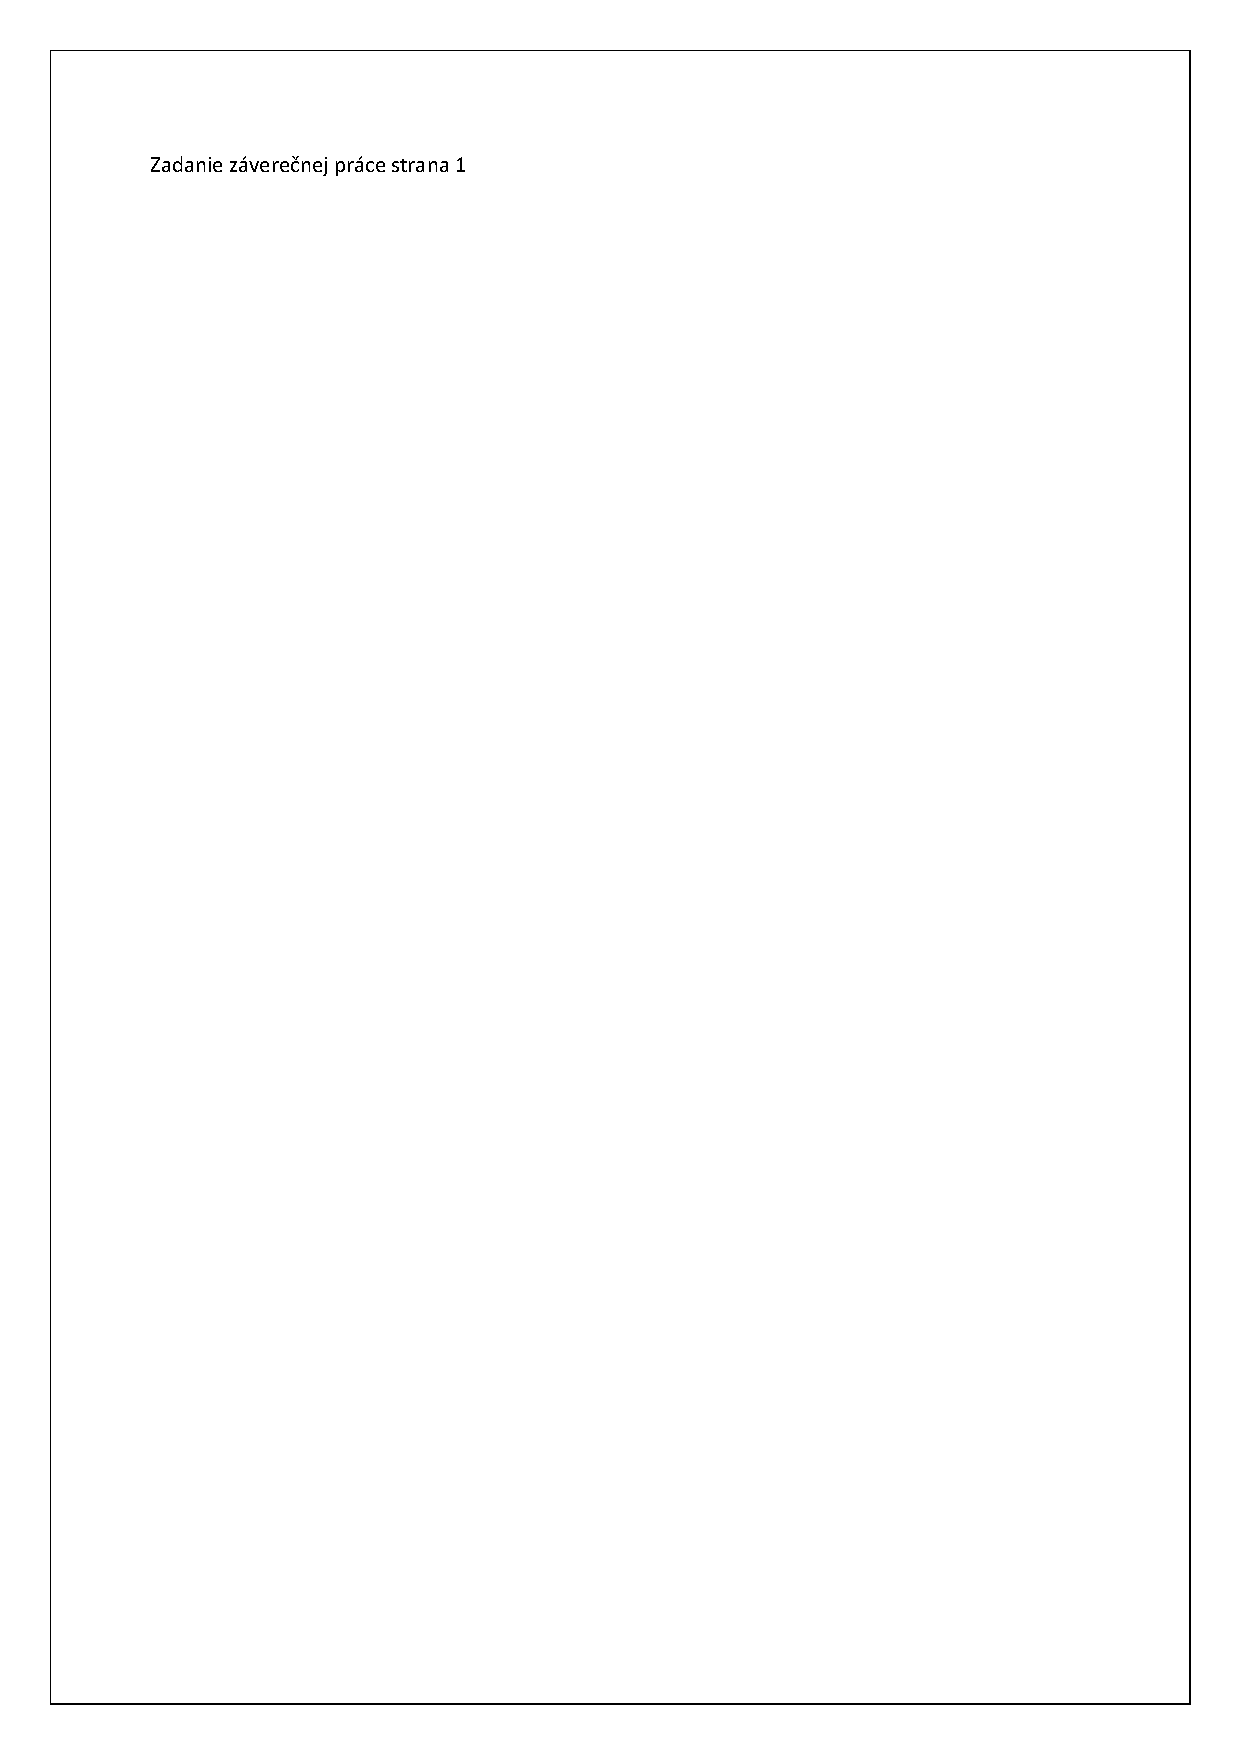
\includepdf[page=2]{content/assignment.pdf}


% do not remove following commands
% do not following commands
\chapter*{\thesisack}
\markboth{}{}
\addcontentsline{toc}{chapter}{\thesisack}
Write here the acknowledgment

\chapter*{Abstract}
\markboth{}{}
\addcontentsline{toc}{chapter}{Abstract}
The different behavior of the real plant and its mathematical description is a relatively well-known issue in the field of automation, which is a serious problem, especially in a situation where we try to ensure optimal operation of the plant. Many scientific publications address this issue, but the solutions they offer are often very complicated to implement or lead to uncertain results. This work brings a new approach to the model--plant mismatch optimization, which is based on hybrid modeling using the method of guaranteed parameter estimation. We decided to demonstrate the functionality of this method on a plant that is represented by a chemostat, because it offers many problems with modeling due to the presence of living organisms. The basic idea is to supplement the discrepancies between the real plant (Monod model) and the inaccurate mechanical model (Haldane model) using data models, which were identified on the data described by these differences.

The results of the experiments showed that hybrid models can be used to optimize the operation of the plant, but  with an iterative approach they are not able to ensure convergence to the real optimal steady state of the plant, only to its immediate surroundings. Unlike the modifier adaptation scheme, the convergence of hybrid models is significantly faster and less sensitive to measurement noise, which is a great advantage for processes with large time constants.

\chapter*{Abstrakt}
\markboth{}{}
\addcontentsline{toc}{chapter}{Abstrakt}
Slovenský abstrakt

\setcounter{tocdepth}{2}
\renewcommand{\baselinestretch}{0.1}\normalsize
\tableofcontents
\renewcommand{\baselinestretch}{1.1}\normalsize

% ----------------------------------------------------------------%
% The Mainmatter !! Do NOT change the structure!!                 %
% ----------------------------------------------------------------%
\mainmatter

% individual chapters should be included via a separate tex file, as shown in 
% here. When working in TexStudio (recomennded tool for Win and Mac) set the 
% main.tex as an Explicit root document, so you can compile even you are
% working on other chapter in other tex file.
%
% Open main.tex THEN click Options-> Root Document -> Set Current Document as
% Explicit Root

% introduction
\chapter*{Úvod}
\addcontentsline{toc}{chapter}{Úvod}
V tomto momente, ako čítate tento text, prebieha okolo nás množstvo procesov, ktoré zabezpečujú fungovanie dnešnej spoločnosti bez toho, aby si to človek vôbec uvedomoval a ťažko povedať, či si ešte dokážeme predstaviť život bez týchto vymožeností. O čom je reč ? Distribúcia elektrickej energie, pitnej vody, plynu, separácia odpadu či čistenie odpadových vôd alebo každodenný prísun potravín, liečiv, pohonných hmôt, oblečenia atď. Asi je zrejmé, že takto by sme mohli pokračovať ešte veľmi dlho. Čo sa však snažíme ozrejmiť je, že väčšina týchto procesov je nejakým spôsobom automatizovaná, čo nám umožňuje vykonávať daný proces efektívne, kvalitne a hlavne bezpečne. 

Základným kameňom väčšiny pokročilejších metód automatizácie je matematický model zariadenia. V princípe existujú dva prístupy k matematickému modelovaniu. Prvý prístup je založený na fyzikálnych zákonoch, ktorý vedie k tak zvaným mechanickým modelom. Problémom takéhoto modelovania je, že s rastúcimi požiadavkami na kvantitu, kvalitu, bezpečnosť alebo efektivitu, rastie aj zložitosť priemyselných procesov -- jednak štruktúra zariadenia a jednak stupeň automatizácie, čo vedie ku komplikáciám. Nehovoriac o tom, že takýto prístup je časovo a aj finančne veľmi náročný. Druhý prístup vychádza z analýzy a identifikácie veľkého množstva nameraných procesných údajov, čo vedie k dátovým modelom. Dátové modely sú jednoduchšie na konštrukciu, avšak môžu so sebou prinášať neistoty v podobe nesprávnej štruktúry modelu alebo parametrov. Tieto neistoty sú najčastejšie spôsobené vplyvom chyby merania.

Existuje viacero metód, ktoré dokážu spracovať zašumený signál, a každá z nich so sebou nesie určité nevýhody. Napríklad metóda najmenších štvorcov predpokladá, že šum merania má normálne rozdelenie a ak tento predpoklad nie je dodržaný, môže viesť k nesprávnym výsledkom.

Garantovaný odhad parametrov (GOP) je metóda, ktorá obchádza problém poznania rozdelenia náhodných veličín a namiesto toho predpokladá ľubovoľnú ale ohraničenú chyba merania. Výsledkom identifikácie pomocou GOP sú intervalové odhady parametrov modelu, ktoré zabezpečia, že nameraný výstup procesu sa bude nachádzať v rozmedzí stanovenej chyby merania.  

Tu sa naskytá otázka, či by nebolo možné opísať komplikované zariadenie jednoduchším mechanickým modelom a vzniknuté rozdiely od skutočného zariadenia doplniť dátovými modelmi. Ako bolo ukázané vo viacerých vedeckých publikáciach, takéto hybridné modely je možné skonštruovať a využiť ich v rôznych oblastiach automatizácie \cite{hamilton:hybrid_modeling:2017}, \cite{hernandez:economics_opt_w_mismatch:2019}. Výhodou hybridných modelov je väčšia robustnosť a krátkodobá predikcia, najmä v situáciách, kde je veľká neistota v parametroch modelu \cite{hamilton:hybrid_modeling:2017}.

Hlavným predmetom tejto práce je ukázať ako možno skonštruovať hybridný model využitím metódy garantovaného odhadu parametrov a aplikovať ho pri ekonomickej optimalizácii dynamického procesu prietokového biochemického reaktora.

Biochemické reaktory sa považujú za dôležitú súčasť chemického priemyslu. Široká škála dôležitých zlúčenín ako farmaceutické produkty, rôzne polyméry alebo produkty potravinárskeho priemyslu sa vyrábajú pomocou určitého fermentačného média (rôzne baktérie, kvasinky, vláknité huby alebo enzýmy) za prísne stanovených podmienok v biochemickom reaktore \cite{srinivasan:chemostat_opt:2003}. Na druhej strane, biochemické reaktory vykazujú širokú škálu dynamického správania a ponúkajú veľa problémov s modelovaním v dôsledku prítomnosti živých organizmov, ktorých rýchlosť rastu je opísaná komplexnými kinetickými výrazmi \cite{psichogios:hybrid_process_model:1992}.


% theory
	%biochem reaktor
	\chapter{Biochemický reaktor}
\section{Základné informácie}

	\section{Rozdelenie biochemických reaktorov}

	\section{Parametre opisujúce biochemický reaktor}

	%matematicke modelovanie
	\chapter{Matematické modelovanie}
\section{Základné mechanické modely biochemického reaktora}



	\section{Analýza matematických modelov}
\subsection{Dynamika}
\subsection{Stabilita}


	%datove modelovanie
	\chapter{Dátové modelovanie}
\section{Dátové modely}



	\section{Hybridné modely}
	\section{Odhad parametrov}
\subsection{Optimalizačné metódy}
\subsection{Prístupy k odhadu parametrov}


	\section{Garantovaný odhad parametrov}

\subsection{Odhad parametrov FIR modelu}

\subsection{Odhad parametrov ARX modelu}


	\section{Verifikácia dátových modelov}
	%ekonomicka optimalizacia
	\chapter{Optimalizácia prevádzky biochemického reaktora}
\section{Prístupy k optimalizácii}

\subsection{Dvojkroková optimalizácia}

\subsection{Modifier Adaptation Scheme}

\subsection{Využitie hybridných modelov}




	
% conclusions
\chapter{Výsledky}
thesis conclusions

% Appendices (Prílohy) comment by "%" if not neccesary
\appendix
\chapter{Resumé}
V oblasti automatizácie sa často stretávame s problematikou nezhody matematického opisu so skutočným zariadením. Tieto nezhody sú väčšinou spôsobené rôznymi aproximáciami, ktorými sa snažíme v jednoduchosti, matematicky opísať správanie komplexného systému. Podobne je to aj v prípade biochemických reaktorov. Vlastnosti biochemických reaktorov sú výlučne stanovené správaním živých organizmov, ktoré ponúkajú široké spektrum dynamického správania. Ich správanie sa líši nielen v závislosti od typu mikroorganizmu, ale aj v rámci jedného druhu, čo vedie k problémom s modelovaním takýchto procesov a v konečnom dôsledku môžeme skončiť s matematickým opisom, ktorý je rôzny od skutočnosti. 

Odlišnosť v správaní skutočného biochemického reaktora a jeho modelu predstavuje závažný problém, hlavne v situácii, keď sa snažíme zabezpečiť efektívnu prevádzku zariadenia. Veľa vedeckých publikácii sa venuje práve tejto tématike, ale riešenia, ktoré ponúkajú, ako napr. dvojkroková optimalizácia alebo úprava účelovej funkcie použitím modifikátora, sú často veľmi komplikované na realizáciu alebo vedú k nepresným výsledkom. Z tohto dôvodu sme sa rozhodli, že navrhneme odlišný prístup k problematike optimalizácie prietokového biochemického reaktora, pomocou nepresného mechanického modelu, ktorý je založený na hybridnom modelovaní s využitím garantovaného odhadu parametrov.

Väčšina metód nerieši problematiku voľby rádu modelu, ktorá je esenciálnou úlohou pri identifikácii dátových modelov a výrazne komplikovanejšou ako odhad parametrov modelu. Garantovaný odhad parametrov nám ponúka informácie o minimálnom ráde (štruktúre) modelu a v spojení s Pareto frontom sme dokázali posúdiť aj kvalitu modelov vyšších rádov. Vhodný rád modelu sme potom zvolili na základe kompromisu medzi presnosťou odhadu modelu a jeho maximálnym rozptylom odhadu. V ďalšej časti identifikácie pomocou GOP sme získali garantovanú oblasť všetkých možných riešení, v rámci stanovenej chyby modelu. Táto oblasť, ktorá je určená minimálnou a maximálnou realizáciou modelu nám zaručuje, že skutočné riešenie leží v vo vnútri.  

Ukázali sme, že takto dokážeme nájsť vhodné dátové modely, či už FIR alebo ARX, na opis údajov, ktoré vyjadrujú rozdiel koncentrácie biomasy alebo substrátu medzi skutočným zariadením (Monod model) a nominálnym modelom (Haldane model). Dynamika týchto modelov bola odlišná, ale v predikcií ustálených stavov boli FIR aj ARX model rovnako dobré. Preto sme sa rozhodli, že pri konštrukcii hybridných modelov sa zameriame iba na FIR modely.

Výsledky experimentov hybridného modelovania nás priviedli k záveru, že hybridné modelovanie môže byť použité na optimalizáciu prevádzky biochemického reaktora. Z dát, ktoré dokážeme získať zo zariadenia, sme odvodili dva hybridné modely, jeden substrátový a druhý biomasový. Oba viedli k rovnakým výsledkom, ak sme upravili vplyv chyby merania koncentrácie biomasy tak, aby bola porovnateľná s chybou merania koncentrácie substrátu, vzhľadom na generované skokové zmeny. Uviedli sme niekoľko prístupov v rámci hybridného modelovania, ktoré sa dajú aplikovať na spomínanú problematiku. Iteračná metóda dokázala skonvergovať v priebehu pár krokov, ale dostala sa iba do okolia optima. Ak sme dátovú časť hybridného modelu natrénovali na dopredu známych dátach, tak sme sa dostali do presného optimálneho stavu zariadenia. Ale ak by sme pridali dáta zo skokových zmien pri väčších hodnotách rýchlosti riedenia, tak s veľkou pravdepodobnosťou by sme optimálny stav presiahli. Nevýhodou tohto prístupu je aj skutočnosť, že ak zapojíme vopred natrénovaný model do iteračnej optimalizácie, tak po niekoľkých iteráciách sa ustálený stav zariadenia vzdiali od optimálneho. Je to spôsobené tým, že po určitom čase už iteračný prístup nedokáže vygenerovať informačne výdatné dáta na identifikáciu dátového modelu. Najdôležitejším výsledkom v rámci hybridného modelovania je, že aj keby hybridný model predikoval presný rozdiel v koncentrácii zariadenia a nominálneho modelu v optimálnom režime, nikdy by sme nedosiahli skutočné optimum zariadenia, ale dostali by sme sa do veľmi blízkeho okolia.

Dvojkroková optimalizácia dokázala v niektorých špeciálnych prípadoch (najmä na začiatku optimalizačného procesu, keď sme mali k dispozícii málo dát) skonvergovať k optimu zariadenia, iba pomocou odhadu kinetických členov nominálneho modelu, pretože zväčšovaním hodnoty inhibičného koeficientu, vieme zmenšiť rozdiely v správaní Monod a Haldane modelu.
V ďalších iteráciách, kedy narastal počet dát, teda sa zvyšovala presnosť odhadu, sa riešenia od optima vzdialili. Problematická situácia nastala najmä vtedy, ak koeficient inhibície $ K_I $ nadobudol hodnoty rádovo $ 10^{10}\si{\gram\per\liter} $. To viedlo k takému priebehu účelovej funkcie nominálneho modelu resp. iba jej časti, ktorá spôsobila problémy pri samotnom riešení optimalizačnej úlohy a výsledkom boli rýchlosti riedenia, ktoré dostali prietokový biochemický reaktor do stavu vymytia.

V teoretickej rovine, je schéma úpravy modifikátora jedinou z použitých metód, ktorá dokáže uviesť zariadenie do jeho optimálneho režimu v niekoľkých krokoch, aj napriek nepresnému matematickému opisu zariadenia. Rýchlosť konvergencie závisí od veľkosti váhového koeficientu $ c $, kde menšie hodnoty znamenajú rýchlejší priebeh konvergencie a naopak väčšie hodnoty pomalší. Situácia sa zmenila, ak sme začali uvažovať vplyv šumu merania. Ako sme ukázali, tak chyba merania mohla v niektorých situáciách pomôcť rýchlejšej konvergencii, ale ak bol šum merania výraznejší ako skoková zmena, vznikali oscilácie a nedokázali sme zabezpečiť konvergenciu k optimu, hlavne v iteráciách, kedy skutočný gradient účelovej funkcie bol rovný nule. Spoľahlivosť tejto metódy záleží na nastavení jej parametrov, čo vôbec nie je jednoduchá úloha, najmä v prípade biochemického reaktora, kde fluktuácia koncentrácie biomasy je veľmi výrazná.

Pri porovnaní jednotlivých metód pre niekoľko rôznych realizácií šumu merania sme zistili, že vo väčšine prípadov si problematikou optimalizácie prevádzky prietokového biochemického reaktora na základe nepresného mechanického modelu najlepšie poradila metóda s použitím hybridného modelovania, i keď od začiatku sme vedeli, že nás dostane iba do blízkeho okolia optima. V dvadsiatej iterácii sa hybridný model aj schéma úpravy modifikátora dostali do približne rovnakého ustáleného stavu. Rozdiel bol v tom, že zatiaľ čo metóde schéme úpravy modifikátora to trvalo celých 20 iterácii, čo v prípade biochemického reaktora predstavuje 1000 hodín, hybridné modely to zvládli za 5 iterácií, teda 250 hodín. Dvojkroková optimalizácia už v druhej iterácii uviedla zariadenie do optimálneho ustáleného stavu, ale v ďalších krokoch divergovala od optima do stavu vymytia.

Iteračný proces optimalizácie pomocou hybridných modelov by sa dal ešte vylepšiť. My sme ukázali, že korekcia ustálených stavov nominálneho modelu, nie je v spojní s iteračným prístupom najvhodnejším adeptom na optimalizáciu prevádzky. Ak by sme pristupovali k optimalizácii, v rámci hybridného modelovania, podobne ako schéma úpravy modifikátora, t.j. zmenou gradientu účelovej funkcie, je tu možnosť, že by sme takto dokázali dosiahnuť presné optimum. Podobne by sme mohli použiť hybridné modely na odhad ustálených stavov zariadenia, pomocou ktorých by schéma úpravy modifikátora vedela omnoho presnejšie odhadnúť gradient účelovej funkcie. Tieto hypotézy by však bolo potrebné overiť ďalším výskumom.

Hybridné modelovanie má niekoľko výhod oproti schéme úpravy modifikátora. Tým, že hybridné modely dokážu predikovať údaje zariadenia, vedeli by sme ich použiť pri riadení procesov, pričom riadenie by bolo omnoho kvalitnejšie ako s použitím samotného nominálneho modelu, čo sme aj demonštrovali na výsledkoch predikčných vlastností modelov. Šum merania nezohráva až takú významnú úlohu pri optimalizácii zariadenia. Dôležitú rolu pri tejto vlastnosti zohráva identifikácia dátových častí hybridných modelov pomocou metódy garantovaného odhadu parametrov. 

Kvalita hybridných modelov je stanovená kvalitou ich dátových častí. Ako sme ukázali, tak lineárne dátové modely ako FIR alebo ARX sa nedokážu efektívne vysporiadať s nelinearitou systému. Z tohto dôvodu vedú aj hybridné modely k nepresnej predikcii. S týmto problémom by sme sa pravdepodobne vedeli vysporiadať zmenou štruktúry hybridného modelu za sériovo--paralelnú, ale toto tvrdenie by bolo nutné overiť, čo môže byť námetom na ďalšiu prácu.

%----------------------------------------------------------------%
%  The Backmatter !! Do NOT change the structure!!               %
%----------------------------------------------------------------%
% Bibliography to TOC
% do not remove
\backmatter
\providebibliography
\bibliography{bibfile}

%----------------------------------------------------------------%
%   The end of the document                                      %
%----------------------------------------------------------------%
\end{document}
